\section{Audio (Sophie)}
\label{sec:audio-sophie}
\subsection{Scoring of apnoea R\&K vs. AASM}
Audio signals taken during polysomnograms are currently scored by sleep specialists. There are two guidelines as to how to do this. The Rechtschaffen and Kales Manual is long standing, it was the only manual in use between 1968 when it was created and 2007 when the AASM Manual came into use. 

The R\&K manual is based on healthy subjects aged 21 to 86 years and does not actually mention how to recognise apnoeas~\cite{rechtschaffen1968manual}. It has also been criticised for being open to interpretation. The AASM manual has a slight change in terminology and changes distribution of NREM sleep stages, but the main difference is it explains how to classify more sleep abnormalities including apnoeas and arousals ~\cite{moser2009sleep}.

The AASM scores a signal as an apnoea if: there is a drop in the peak thermal sensor excursion by more than 90\% of baseline, the event lasts at least 10 seconds and at least 90\% of the event’s duration meets the amplitude reduction criteria for apnoea. Obstructive apnoeas are associated with continued or increased inspiratory effort through the period of absent airflow. A minimum desaturation criterion is not required. The basis for scoring arousals is based on EEG and EMG and therefore is not helpful in terms on how to analyse audio signals ~\cite{iber2007aasm}.

Both of these guidelines are used by modern papers and so awareness of both is needed. Given both result in scoring of apnoeas, choking events and snores they are useful as they lead to labelled signals which can be used for training and testing data sets.
\subsection{Methods of analysis}
The aim of the audio analysis is to find and count the apnoea-choking events to directly determine AHI, or use the difference in snoring type between OSA sufferers and simple snorers as an indicator of AHI. The initial process of this in the majority of the analyses is to split the signal down into intervals of time of somewhere between 10 and 30 seconds and assess the features of those intervals independently to determine whether they contain apnoea, choking, snoring, breathing or something else.

The starting point for assessing the intervals will be speech analysis, as snoring and speech are both generated in the vocal tract, although snoring is caused by vibration of the pharyngeal structures during inspiration whereas speech is vibration of the vocal cords during expiration. The digitalisation and filtering of the signals will be mainly performed by inbuilt phone software, so the focus here will be on which feature to extract, how to extract them and classification of the features. 

\subsection{Frequency of Prominent Peaks}
Using Fast Fourier Transforms a power spectrum can be created of the snores. This can then be characterised in a number of ways including establishing: Fa the fundamental frequency; Fo the lowest frequency; Fpeak the frequency with the maximum power; and Fmean the statistical mean frequency. Fmax, the highest observed frequency, can also be calculated, however there are different conventions for this: in all cases it is defined as the frequency beyond which the signal amplitude has dissipated to less than a percentage of its peak power, however some studies use 3\%, whereas others use 10\%. 

Perez-Padilla et al used Fa, Fo, Fpeak and Fmax to examine the differences between nine OSA sufferers and ten simple snorers, defining Fmax as dissipating to 3\% of peak power. Sound was recorded via a microphone attached to the manubrium sterni (chest). Significant variation was found between snores in a given patient making it hard to find a differentiator between OSA sufferers and simple snorers. It was found that for OSA suffers Fpeak was usually at a higher frequency than Fa, however this was not significant enough to be used to differentiate the two groups ~\cite{whitelaw1993characteristics}.

Fiz et al used Fpeak, Fmean and Fmax defined at 10\% of peak power, to distinguish between ten OSA sufferers and seven simple snorers. The microphone was placed just above the larynx without skin contact. Two features were found to distinguish OSA sufferers from simple snorers. The first was peak frequency (Fpeak) which was significantly lower in OSA sufferers. All but one OSA sufferer had an Fpeak below 150Hz and all but one non-OSA sufferer has an Fpeak about 150Hz. A strong non linear negative correlation was also seen between Fpeak and the number of AHI events as seen in Figure \ref{fig:Fiz1996fig3}; this is associated with a Spearman rank order correlation: r=-0.70; p\textless0.0016. The second feature was to do with the shape of the power spectrum. The simple snorers displayed a clear fundamental frequency and harmonic pattern whereas the OSA sufferers displayed a low frequency peak with scattered peaks over a narrow band of frequencies; Figure \ref{fig:Fiz1996fig12} shows the different patterns. Fiz et al attributed the differences seen to microphone placement, Perez-Padilla et al placing their microphone on the chest whereas Fiz et al placing above the larynx, this results in a different filtering effect caused by the different tissues and cavities the sound travels through ~\cite{fiz1996acoustic}.

Prominent peaks alone are not sufficient to diagnose obstructive sleep apnoea. 
\begin{figure}[h]
\centering 
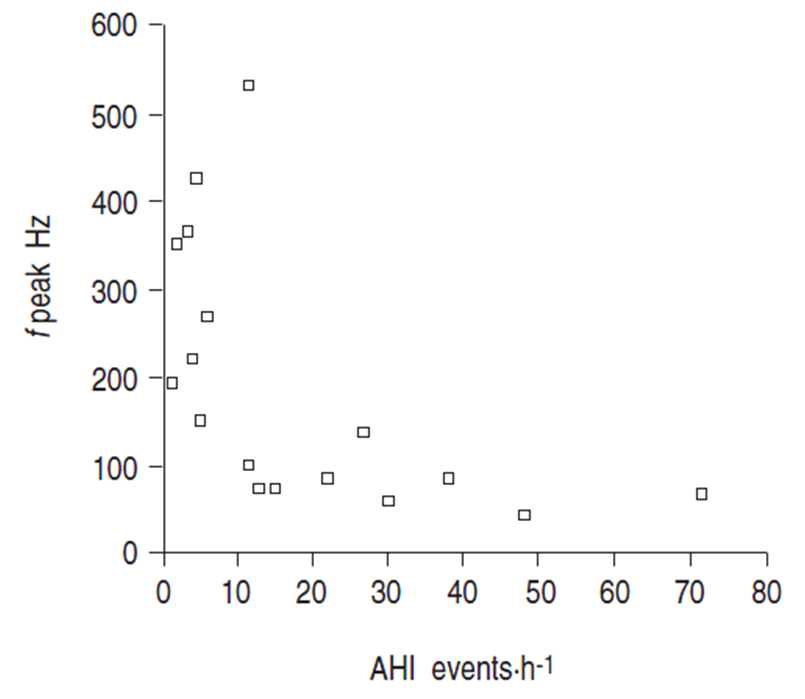
\includegraphics[width=0.3\textwidth]{drawings/Fiz1996fig3}
\caption{Relationship between apnoea/hypopnoea index (AHI) and
peak frequency (Fpeak) of spectrum in seven simple snorers and 10
obstructive sleep apnoea (OSA) patients. There is a significant negative correlation (Spearman rank
order correlation: r=-0.70; p\textless0.0016) ~\cite{fiz1996acoustic}.}
\label{fig:Fiz1996fig3}
\end{figure}
\begin{figure}[h]
\centering 
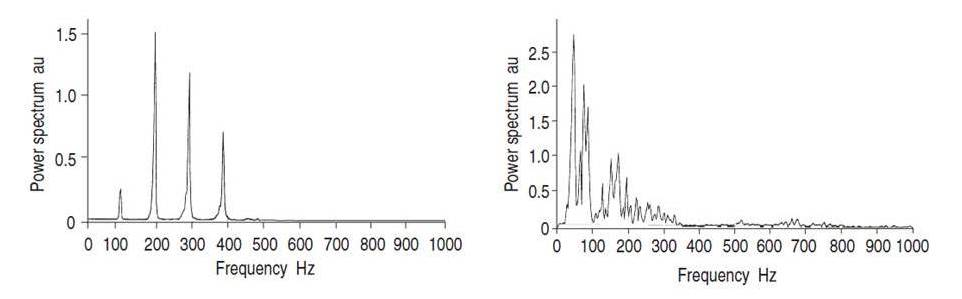
\includegraphics[width=0.7\textwidth]{drawings/Fiz1996fig12}
\caption{Power Spectrum of first breath from a simple snorer and OSA patient ~\cite{fiz1996acoustic}.}
\label{fig:Fiz1996fig12}
\end{figure}


\subsection{Power Ratio}
Given the difference in spectra between those with OSA and simple snorers, there is potential to characterise this by means of a cumulative power ratio. This would be the area under one part of the power spectrum divided by the area under the rest. Where the threshold is placed would depend on what characteristic was trying to be differentiated. 

Perez-Padilla et al used superimposed spectra from ten snores from each subject (9 OSA, 10 simple snorers) and a threshold of 800Hz, dividing the integral of the spectra above 800Hz with that below 800Hz. For OSA patients who took a second breath after an apnoea the cumulative power ratio was also calculated for that. Figure \ref{fig:Perez1993fig8} shows the scattering of the ratios, with simple snorers having a ratio of 0.08$\pm$0.02 and OSA sufferers a ratio of 1.12$\pm$0.31. A threshold of 0.3 was proposed which would distinguish all but one OSA sufferer on first breath after apnoea, this patient had a low AHI and mild symptoms ~\cite{whitelaw1993characteristics}

\begin{figure}[h]
\centering 
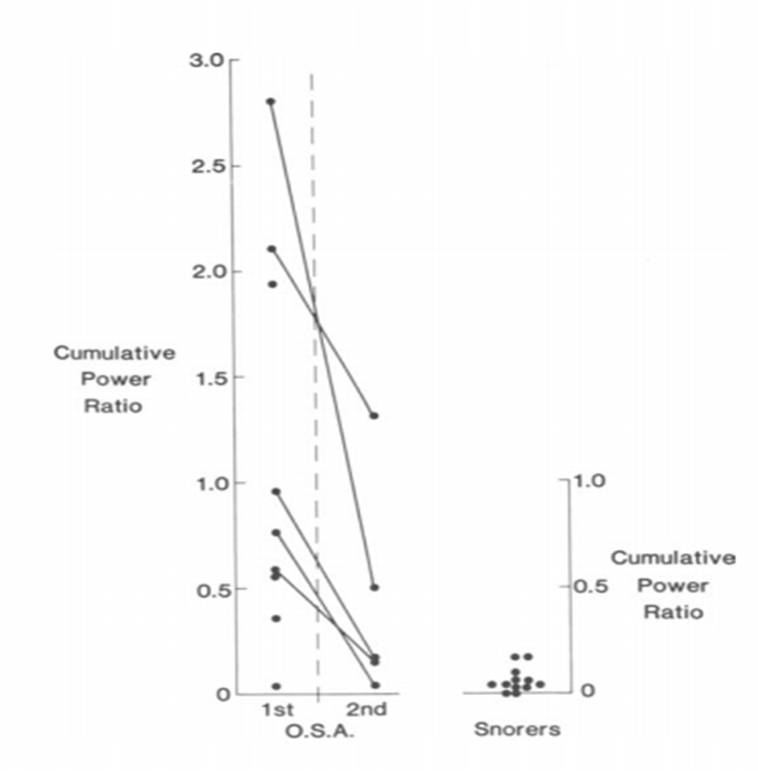
\includegraphics[width=0.3\textwidth]{drawings/Perez1993fig8}
\caption{Cumulative power ratio between frequency components higher and lower than 800 Hz in patients with OSA and in snorers ~\cite{whitelaw1993characteristics}.}
\label{fig:Perez1993fig8}
\end{figure}

Hara et al used the same method as above on 46 OSA sufferers and 12 simple snorers, keeping the threshold at 800Hz, but using a ratio of below 800Hz to above 800Hz (the inverse of the ratio used by Perez-Padilla et al). Simple snorers had a power ratio of 34.002 (0.03 when defined as in the Perez-Padilla study) whereas OSA sufferers had a ratio of 6.288 (0.16 when defined as in the Perez-Padilla study). The p value of a Mann-Whitney U test was 0.015; this small value is a good indicator that this did not happen by chance ~\cite{hara2006acoustic}. 

Hara et al would not recommend this approach as the calculation is very time consuming ~\cite{hara2006acoustic}. Significant differences were found between the values of the ratios in both studies although in both cases a difference between OSA sufferers and simple snorers was clearly seen. 
\subsection{Sound Intensity}
Sound intensity can be used for diagnosis in a couple of ways; as a cut off for distinguishing between snores and apnoeas in order to look for apnoea-arousal events, and as a distinguisher between apnoeic snores and non-apnoeic snores. In both cases frequency need not be known, although in the first approach the signal does need to be split into temporal intervals. 

Van Brunt et al defined an acoustic signature event as an apnoeic event lasting between 10 and 90 seconds followed by snoring. Where apnoea had an intensity below 50$\mu$V and snoring above 100$\mu$V. 30 second intervals were analysed by sound intensity and polysomnogram and considered in two ways: firstly each patient (69 patients, 51 OSA suffers, 18 not) was assessed independently and RDI score compared with predictions. For an RDI of 15/hour or greater, sensitivity was 93\%, specificity 25\%, false positive 36.2\%, false negative 2.8\%, 60.9\% classified correctly. Secondly pooling all the observations (60231) resulting in a 33\% sensitivity, 98\% specificity, and 85\% classified correctly ~\cite{van1997intensity}.

Wilson et al looked at four sound intensity levels:$ L_{1}, L_{2}, L_{3}$ the dB levels exceeded for 1\%, 5\% and 20\% of the test period respectively, and $L_{eq}$ the average dB level. 1139 patients were studied (682 OSA, 261 simple snorers and 196 unknown). Differences were seen between the sound intensity of apnoeic and non-apnoeic snores with non-apnoeic snores having a lower intensity as seen in Table \ref{table:wilson}. A logistic regression model with RDI $\geq$ 10 as the dependent variable found a cut off of $L_{eq}$ $\geq$ 38 to be significant, with a regression coefficient of 1.24, a standard error of 0.28 and an odds ratio of 3.44 (95\% CI) ~\cite{wilson1999snoring}.

\begin{table}[h]
\centering
\begin{tabular}{c c c}
\toprule
Sound Intensity Measure&Nonapnoeic Snoring (RDI \textless 10)&Apnoeic Snoring (RDI $\geq$ 10)\\ \midrule
$L_{eq}$, dBA&42.7 (42.0–43.4)&48.8 (48.7–49.3)\\ 
$L_{1}$, dBA&53.4 (52.8–54.1)&59.2 (58.7–59.7)\\ 
$L_{5}$, dBA&48.0 (47.4–48.6)&53.2 (52.7–53.7)\\ 
$L_{10}$, dBA&46.0 (45.5–46.5)&50.4 (49.9–50.9)\\ \bottomrule
\end{tabular}
\caption{Sound Intensity Measures for Subjects With Apnoeic Snoring (RDI $\geq$ 10) and Non-apnoeic Snoring (RDI \textless 10).}
\label{table:wilson}
\end{table}
\subsection{Formants}
Formants are the resonant frequencies of the signal, most easily determined by picking out the peaks on a linear predictive coding (LPC) spectrum of the signal. LPC is the spectral envelope produced by a linear predictive model. The lowest formants are associated with degree of constriction of the pharynx, degree of advancement of the tongue and degree of lip rounding respectively, these are often referred to as F1, F2 and F3. Because these physical properties change in sufferers of OSA there is a chance that the frequencies associated with them will change too. Threshold frequencies to distinguish OSA sufferers and simple snorers are therefore sought. 

Sola-Soler et al used formant frequencies to distinguish between snores from eight simple snorers (447 snores) and eight OSA sufferers (236 normal snores and 429 post-apnoeic snores). The spectral envelope was estimated by linear predictive autoregression, with very low amplitude spurious peaks rejected by a 3dB threshold. Investigation of the spectral envelope found 2 to 6 formants in each snore, these fell in common frequency ranges around 150Hz, 500Hz, 1KHz, 1.7KHz, and in a few snores 2.2KHz. This led to definition of five frequency bands: B1[0,300), B2[300,700), B3[700,1400), B4[ 1400,1900) and B5[ 1900,2500) in Hz. For each band and type of snore (simple snorer SN, OSA normal snore OP-N, and OSA post apnoeic snore OP-PA) the mean value Fi and standard deviation SFi was calculated. Table \ref{table:sola2003formants} shows a comparison between these means and standard deviations for each combination of snore type calculated using the Mann-Whitney U test (the fifth band was left off because so few snores exhibited this formant). If a snore had more than one formant in a band the average frequency of those was used in the calculation. Bands 1 \& 3 showed significant differences between formants when comparing the standard deviation of simple snorers and OSA sufferers both in normal snores and post apnoeic snores of the OSA sufferers. The most distinct difference was between the standard deviation of simple snorers’ normal snores and post-apnoeic snores in band 1 which had a probability of 0.0006 ~\cite{sola2003spectral}.

\begin{table}[h]
\centering
\begin{tabular}{l c c c c c c c c}
\toprule
Contrasted populations&F1&SF1&F2&SF2&F3&SF3&F4&SF4\\ \midrule
SN 1 OP-N&0.4179&0.0151&0.0882&0.0618&0.1556&0.0045&0.5839&0.8551\\ 
SN / OP-PA&0.7104&0.0006&0.1061&0.6389&0.5338&0.0012&1.0000&0.1255\\ 
OP-N 1 OP-PA&0.6434&0.0372&0.4822&0.0842&0.5628&0.2030&0.6310&0.1495\\ \bottomrule
\end{tabular}
\caption{Bilateral significance in Mann Whitney U test to contrast population difference.}
\label{table:sola2003formants}
\end{table}
Ng et al tested 30 OSA sufferers and ten simple snorers and found a threshold for F1 of 470Hz, but no significant threshold for F2 nor F3. This threshold yielded a sensitivity of 88\% and a specificity of 82\%. However increased sensitivity and specificity were seen if different thresholds were used for men and women as seen in Table \ref{table:ng2008aformantstable1}. Women show a greater distinction in F1 frequency than men as well as a reduced spread of results, although more outliers amongst the simple snorers, as seen in Figure \ref{fig:ng2008afig1}. It is however worth noting that the sample size for women was small (6 OSA sufferers, 4 simple snorers). Once the threshold has been established an equation is needed to convert it to an AHI value. A number of equations were proposed and regression used to see which was the best fit, as seen in Table \ref{table:ng2008aformantstable2}. A power law came out best with a regression of 0.5334 giving a predicted AHI score of 12.2 when 10 was being aimed for. It is worth noting that the same subjects were used for training and testing, although different data for each ~\cite{ng2008could}.

\begin{figure}[h]
\centering 
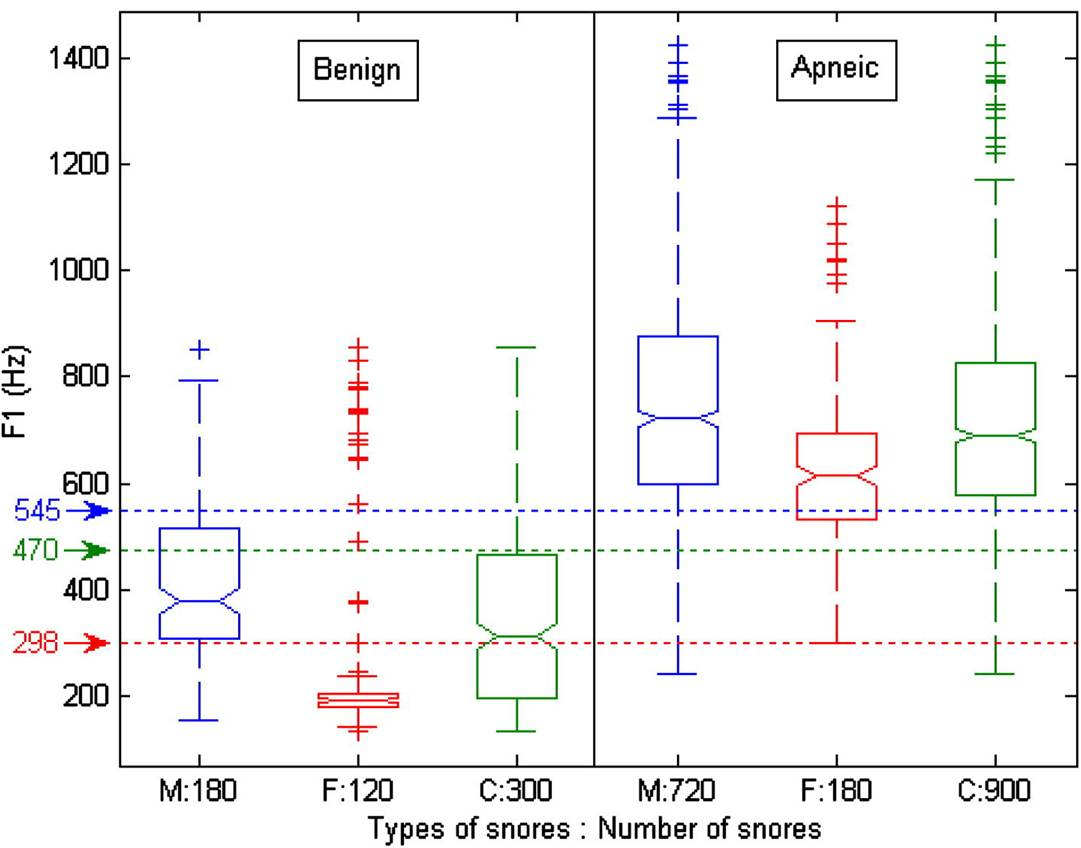
\includegraphics[width=0.5\textwidth]{drawings/ng2008afig1}
\caption{Notched box plots of apnoeic and benign snores in the training dataset for males (M), females (F), and for both males and females combined (C), under first formant frequency (F1) analysis, with marked threshold values, from Table \ref{table:ng2008aformantstable1} ~\cite{ng2008could}.}
\label{fig:ng2008afig1}
\end{figure}
\begin{table}[h]
\centering
\begin{tabular}{c c c c c c c c c}
\toprule
Type&AHI&Data size (train ; test)&F1&F2&F3&Threshold of F1 (AUC : F1; F2; F3)&Sens&Spec\\ \midrule
M:A&52.8$\pm$24.7&720 ; 240&750$\pm$204&1842$\pm$238&3008$\pm$266&545&\multirow{2}{*}{83}&\multirow{2}{*}{92}\\ 
M:B&5.3$\pm$3.5&180 ; 60&425$\pm$157&1670$\pm$271&2858$\pm$405&(0.8977; 0.6860; 0.6117)&&\\ 
F:A&23.6$\pm$15.1&180 ; 60&623$\pm$150&1676$\pm$303&2739$\pm$282&298&\multirow{2}{*}{100}&\multirow{2}{*}{95}\\ 
F:B&3.4$\pm$3.2&120 ; 40&263$\pm$187&1564$\pm$294&2813$\pm$297&(0.8969; 0.5894; 0.5850)&&\\ 
C:A&46.9$\pm$25.7&900 ; 300&724$\pm$201&1809$\pm$261&2955$\pm$290&470&\multirow{2}{*}{88}&\multirow{2}{*}{82}\\ 
C:B&4.6$\pm$3.4&300 ; 100&360$\pm$187&1627$\pm$285&2840$\pm$366&(0.8992; 0.6820; 0.5964)&&\\ \bottomrule
\end{tabular}
\caption{AHI, apnoea–hypopnoea index (events/h); Data size, number of snores; AUC, area under receiver operating characteristic curve; Sens, sensitivity (\%); Spec, specificity (\%).}
\label{table:ng2008aformantstable1}
\end{table}
\begin{table}[h]
\centering
\begin{tabular}{c c c c}
\toprule
Regression&Equations&R2&Predicted AHI/h\\ \midrule
Linear&AHI = 0.0738 (F1) − 10.4067&0.3449&24.3\\ 
Quadratic&AHI = − 0.0001 (FI)2 + 0.1778 (F1) − 39.2095&0.3824&26.3\\ 
Logarithmic&AHI = −212.4891 + 89.9464 Log (F1)&0.3553&27.9\\ 
Exponential&Log (AHI) = 0.1545 + 0.0018 (F1)&0.4602&10.3\\ 
Power&Log (AHI) = −5.2100 + 2.3565 Log (F1)&0.5334&12.2\\ \bottomrule
\end{tabular}
\caption{Regression analysis for apnoea–hypopnoea index (AHI) in events/h and first formant frequency (F1) in hertz \\ AHI computed at F1 = 470 Hz. Ideally predicted AHI = 10 events/h.}
\label{table:ng2008aformantstable2}
\end{table}
Yadollahi et al used formant frequencies to distinguish between snores and breaths rather than simple snorers and OSA suffers, so a direct comparison of method cannot be made, however there is value in exploring the method used. Bands were used as in the Sola-Soler study but at different frequency ranges, [20−400]Hz, [270−840]Hz, [500−1380]Hz, [910−1920]Hz, [1680-2680]Hz, [2580-3770]Hz and [3590-5000]Hz these were found using K–means clustering. This is a method of partitioning data unsupervised; it uses an iterative method to find a predefined number of partitions, in this case seven; an error margin of 10^{−5} was used for the iterations. The process is sensitive to initial conditions so was repeated 20 times with different initial conditions, the one with the minimum error was selected. Table \ref{table:yadollahi2009formant} shows the student t-test p values, which show the first and third formants to be significant, with probability p = 0.003 and p = 0.0244 respectively. The F1 frequency of the breath sound was greater than that of the snore while the F3 frequencies were the converse ~\cite{yadollahi2009formant}.

\begin{table}[h]
\centering
\begin{tabular}{c c c c c}
\toprule
Formants&F1&F2&F3&F4\\ \midrule
p-value&0.0003\*&0.1793&0.0244\*&0.7009\\ \bottomrule
\end{tabular}
\caption{Results of P-values of t-test between formants of snore and breath sounds. \* represents the significant values.}
\label{table:yadollahi2009formant}
\end{table}
\subsection{Sub-band Energy Analysis}
This uses the vertical box control chart to segment the signal temporally into intervals. This is a nonparametric detection rule which uses a moving vertical trimmed box, hence the name ~\cite{vbox}. The ten dimensional 500Hz sub-band energy features are computed and then reduced to two dimensional feature space by principal component analysis. This is a statistical procedure that uses orthogonal transformations and results in the largest possible variance within the first component. Classification can then be performed on this 2D feature space to separate the desired classes. 

Cavusoglu et al computed the normalised 500Hz sub-band energy distribution for ten apnoeic snorers and eighteen simple snorers and used principle component analysis to reduce it to two dimensional feature space in order to find the most discriminant features. Robust linear regression was used to separate snores from non-snores. This had a sensitivity of 89.3\% and a specificity of 96.3\% ~\cite{cavusoglu2007efficient}.

Azarbarzin et al used a similar method to Cavusoglu except that K-means clustering was used as the classifier for the thirteen apnoeic snorers and seven simple snorers. When the classification was compared to manually annotated signals, a sensitivity of 94.8\% and a specificity of 96.3\% was found for the distinction between snores and non-snores in OSA sufferers ~\cite{azarbarzin2010unsupervised}.
\subsection{Bispectral Analysis}
Bispectral analysis exploits the fact that the bispectrum reveals both amplitude and phase information about a spectrum, while also being calculated by convolution, makes it the easiest polyspectra to compute. Polyspectra are Fourier Transforms of cumulants, for example the Power Spectrum is the Fourier Transform of the second order cumulant: autocorrelation.  The third-order cumulant $C(m,n)=E\{x(k)x(k+m)x(k+n)\}$ transforms via a Double Discrete Fourier Transform (DDFT) to the bispectrum $B(\omega_1,\omega_2) = E\{X(\omega_1)X(\omega_2)X^*(\omega_1+\omega_2)\}$. Although the bispectrum is often plotted on a square it is symmetric and so only a triangular region is needed to completely describe it, this is defined by $ 0\leq \omega_2 \leq \omega_1, \omega_1 + \omega_2 \leq \pi $.

Quadratic phase coupling (QPC) occurs uniquely in second-order non-linear systems, and is where the phases add and subtract along with the frequency components ~\cite{rastogi2005quadratic}. QPC causes peaks in the bispectrum triangular region, this shows energy is produced at frequency $\omega_1 + \omega_2$, and a flat bispectrum at $\omega_1$ and $\omega_2$ suggests no activity and that it is not affected by QPC. 

Ng et al exploited the bispectrum shape in order to distinguish between nine OSA sufferers and seven simple snorers. The bispectrum was plotted (Figure \ref{fig:ng2007fig45}) and inspected visually, the axes have been normalized with a frequency of 1 being 11025Hz. From visual inspection it appears for simple snorers the biggest peak is near the origin while for apnoeic snores it is further away. This suggests a greater degree of phase coupling in apnoeic snores due to nonlinearities in the signals ~\cite{ng2007bispectral}.

\begin{figure}[h]
\centering 
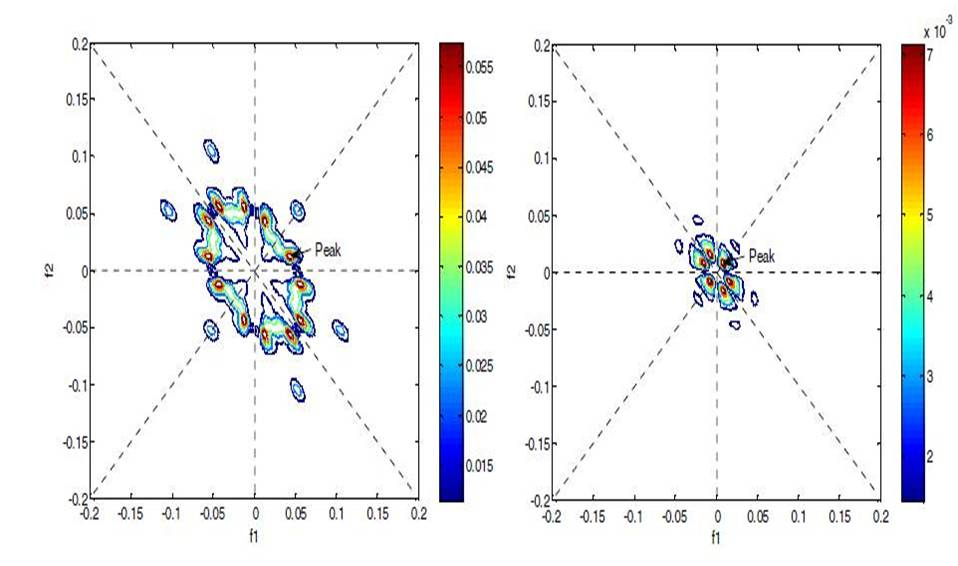
\includegraphics[width=0.7\textwidth]{drawings/ng2007fig45}
\caption{Bispectrum of a common benign snore ~\cite{ng2007bispectral}.}
\label{fig:ng2007fig45 }
\end{figure}

Clustered multiple comparison graphs were then produced, Figure \ref{fig:ng2007fig6}. QPCs appear mainly at f1=f2 for simple snores whereas they appear mainly at f1$\neq$f2 for apnoeic snores. However there is less self coupling; 77\% of simple snores are self coupled compared to 49\% of apnoeic snores. So the analysis shows there are three differences between simple snores and apnoeic snores: apnoeic snores have strong presence of nonlinear interaction, less self-coupling and QPC peaks appear at higher frequencies. 

\begin{figure}[h]
\centering 
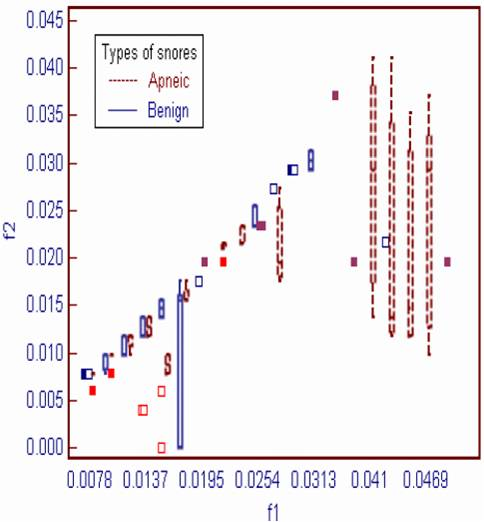
\includegraphics[width=0.5\textwidth]{drawings/ng2007fig6}
\caption{Clustered multiple comparison graphs ~\cite{ng2007bispectral}.}
\label{fig:ng2007fig6 }
\end{figure}

\subsection{Wavelet Analysis}
Wavelet analysis is based on basis functions much like Fourier transforms (they do not have to be orthogonal although they often are), however wavelets are used rather than sines and cosines. As wavelets decay rapidly with time they can be used as a function of time as well as frequency.

Ng et al in 2008 used a special type of discrete wavelet transform (which is time invariant) to distinguish between 30 OSA sufferers and ten simple snorers. Ten snores of about 6 seconds were randomly chosen from each snorer and marked by polysomnogram technologists. Figure \ref{fig:ng2008bfig5} compares the energy approach used by Cavusoglu et al and the time invariant discrete wavelet transform (TIDWT) approach used by Ng et al in this study. At the narrowest tolerance of 25ms the TIDWT approach detected 51\% of the snore segments correctly compared with 8\% for the energy approach, and at the largest tolerance of 125ms the TIDWT approach detected 98\% correctly, whereas the energy approach only managed 87\%, i.e. the TIDWT approach is at least 10\% more effective ~\cite{ng2008snore}.


\begin{figure}[h]
\centering 
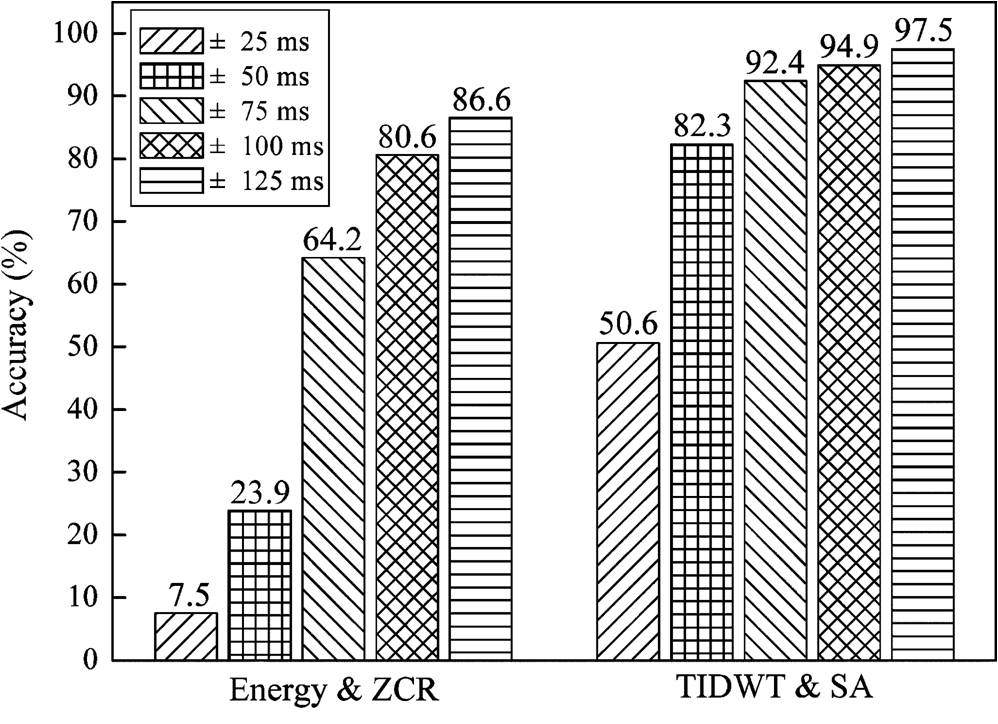
\includegraphics[width=0.5\textwidth]{drawings/ng2008bfig5}
\caption{Accuracy comparisons between conventional- (energy and ZCR) and wavelet-based (TIDWT and SA detector) approaches in snore segment boundary detection at several tolerance degrees: 25, 50, 75, 100, and 125 ms ~\cite{ng2008snore}.}
\label{fig:ng2008bfig5}
\end{figure}

Ng et al in 2009 used continuous wavelet transform in the form of wavelet bicoherence analysis. Bicoherence is the normalised bispectrum and a measure of the amount of phase coupling in a signal ~\cite{van1995wavelet}. Apnoeic snores showed phase coupling at higher frequency modes than benign snores, with apnoeic snores being 20\% less self coupled that benign snores. Two markers were proposed, these were peak frequency component at $f_1$ (PF1) and peak sum frequency (PSF) i.e. the frequencies with the highest coupling strength of frequency 1 and the sum of frequencies 1 and 2. The relationship between the markers and AHI was assessed using various regression models the most successful of which were exponential and power models using residual standard deviation statistic. These produced optimal thresholds for the markers of PF1 = 285 Hz and PSF = 492 Hz resulting in a sensitivity of 85.0\% and a specificity of 90.7\% ~\cite{ng2009investigation}.

\subsection{Multiclass Classification}
Rather than looking at each potential feature separately, as has been done so far, it is possible to use regression analysis and Bayes classifiers (a type of machine learning), amongst others, to predict AHI level from a sound signal without  the need to count the number of apnoeas, instead looking at the overall shape of the signal.

Ben-Israel et al investigated the use of five classifiers on 60 training patient sets and 30 testing patient sets. The features were: Mel-Cepstability, a measure of stability of the spectrum over the whole night; running variance, a measure of the energy variability between snores over the whole night; apnoeic phase ratio, the percentage time the upper airway collapsed using an energy threshold; inter event silence, a count of apnoeic events based on energy patterns; and pitch density, a measure of stability of fundamental frequencies. This resulted in a five dimensional feature vector, which was classified by a Gaussian Bayes classifier. A threshold of AHI \textgreater 10 resulted in a sensitivity of 87\% and a specificity of 80\% ~\cite{ben2012obstructive}.

Sola-Soler et al classified their subject into three classes: $C_{1}$ simple snorers with AHI \textless 5, $C_{2}$ mild to moderate OSA sufferers 5 $\leq$ AHI \textless 30, and $C_{3}$ sufferers of severe OSA with AHI $\geq$ 30. There were 13 simple snorers, 11 $C_{2}$ and 12 $C_{3}$ sufferers. 22 features were used which fell into the categories of sound intensity, pitch, frequency parameters and formants. These were then classified in two main ways: logistic regression and Bayes rule. A forward stepwise selection algorithm was used to find optimum independent variables for two binary logistic regression classifiers used simultaneously; two classifiers were needed because there are two thresholds ~\cite{sola2012multiclass}.
Three different types of naive Bayes classifier were investigated. The optimum independent variables were found by a sequential floating forward selection algorithm up to a maximum of ten variables. The three approaches were Gaussian, kernel diffusion and kernel density, with kernel density producing the best results. Gaussian produced the worst results for the training set probably because snore features are not Gaussian. Bayes using kernel density performed better than logistic regression with accuracy of 83.3\% and 0\% false negatives whereas logistic regression was 72.2\% and 8.3\% respectively ~\cite{sola2012multiclass}.
\subsection{Conclusion}
As has been shown a number of features can be used successfully to differentiate obstructive sleep apnoea sufferers from simple snorers with sub-band energy analysis and multiclass analysis performing the best. There were three ways the signals were classified: regression, K-means clustering and Bayes classifiers. Bayes classifiers and K-means clustering consistently outperformed regression classifiers. These are types of machine learning, although not the only types to be used for the classification of signals used in the diagnosis of OSA. Other types of machine learning used include: Hidden Markov Models used by Rossow et al to classify EEG signals ~\cite{rossow2011automatic}; Support Vector Machines used by Gederi and Clifford to classify images ~\cite{gederi2012fusion}; and neural networks used by Roberts and Tarassenko to classify EEG ~\cite{roberts1992new}. Given the success of machine learning in the cases shown, even with very small training and testing sets, this will be the focus of the next stage of our work. 

